\documentclass[runningheads]{llncs}
\usepackage[T1]{fontenc}
\usepackage{amsmath,amssymb,graphicx,booktabs,array}
\usepackage[hidelinks]{hyperref}
\usepackage{listings}
\setlength{\emergencystretch}{1em}
\newcommand{\E}{\mathbb{E}}
\newcommand{\Prb}{\mathbb{P}}
\newcommand{\calP}{\mathcal{P}}
\newcommand{\OPT}{\mathrm{OPT}}
\begin{document}
\raggedbottom
\title{RecordBatch: Exact Sequential Batch Testing\\under Unknown Dependence}
\titlerunning{Exact Sequential Batch Testing under Unknown Dependence}
\author{Shivam Gupta}
\authorrunning{S. Gupta}
\institute{Independent Researcher, India\\\email{shivam20406@iiitd.ac.in}}
\maketitle
\begin{abstract}
Sequential batch testing evaluates mandatory checks and stops at the first
failing batch. We study additive test costs and a fixed setup charge when
marginal pass probabilities are known but dependence is unrestricted.
A classical comonotonic coupling simultaneously maximizes every policy's
expected cost. We establish an optimal-policy normal form: strictly decreasing
singleton probability records followed by one residual batch. It yields an
exact algorithm with $O(n^2\log n)$ arithmetic operations and $O(n)$ auxiliary
storage. At zero setup, a specialized algorithm takes $O(n\log n)$ operations,
and splitting a robust-optimal residual batch weakly reduces cost on every
outcome. We show unbounded robust loss from independence-optimal scheduling
and strong NP-hardness with batch capacity; a three-test example also shows
that the normal form fails under any positive nominal-objective weight.
Subset optimization and explicit joint-distribution linear programs check
the implementation. Across 480 synthetic instances, median worst-case savings
over exact independence-designed schedules reach 16.2\% at positive setup.
Zero-setup refinement reduces the median independent-law premium from 49.64\%
to 0.01\%. Chronological industrial-log replay shows a zero median held-out
premium after refinement but substantial positive-setup losses. The contribution
is exact optimization under a specific information model, with explicit
computational and operational boundaries.
\keywords{Sequential batch testing \and Distributionally robust optimization
\and Constraint programming \and Dependence uncertainty}
\end{abstract}

\section{Introduction}
Many operational decisions require a conjunction of checks: a software release
must pass its required tests, a data product must satisfy its validation rules,
or an automated workflow must clear its prescribed gates. A failed check can
reject the candidate immediately. Successful checks cannot replace the remaining
ones. Running checks in batches creates a scheduling tradeoff. A batch pays one
setup charge but commits to all its tests before the next stopping decision.
Singleton batches provide more opportunities to stop, at the cost of repeated
setup.

The dependence model changes this tradeoff. Independent failures make
successive checks progressively reduce the probability of continuation.
Correlated failures may leave much less information in a successful check.
In practice, marginal pass rates may be available when a credible joint model
is not: checks can share dependencies, failure causes, or execution contexts.
This motivates the following question:
\emph{Can a batch-testing policy be optimized exactly when its marginal pass
probabilities are fixed but all dependence structures are possible?}

For the model considered here, the answer is yes. The adversarial evaluation
itself follows a classical dependence result. Every prefix survives with
probability at most the smallest marginal in that prefix, and one shared-uniform
coupling attains all these bounds simultaneously. The new structural step is
that only singleton checks setting a new probability record need precede the
final batch. Checks that do not improve a record can be deferred. This converts
optimization over ordered set partitions into a family of shortest-path
problems. Their predecessor costs are affine functions, giving a lower-envelope
implementation with $O(n^2\log n)$ arithmetic complexity.

We call the resulting optimizer \emph{RecordBatch}. The name describes its policy
structure rather than a new dependence inequality. Our contributions are:
\begin{enumerate}
\item an optimal-policy normal form and an exact polynomial algorithm for
unrestricted additive-cost batch testing under fixed marginal information;
\item an unbounded gap for independence-designed policies, together with
interval-uncertainty and marginal-perturbation guarantees;
\item a capacity counterexample, a strong NP-hardness reduction, and a
CP formulation for that extension; and
\item reproducible exact-oracle checks, synthetic experiments, scaling
measurements, and chronological industrial-log replay that quantifies the
price of the ambiguity model.
\end{enumerate}
The replay is deliberately a test of operational limitations as well as of
potential value. Robust optimality under unrestricted dependence does not
imply lower expected cost under the dependence occurring in a particular
deployment.

\paragraph{Scope.}
Each check is perfect, its Boolean outcome is fixed during an episode, and
every check is mandatory on the all-pass path. A failed batch terminates
evaluation; an all-pass batch is the only observation permitting continuation.
Costs represent additive committed work, not parallel makespan. Tests within
a batch cannot be cancelled after one of them fails. The model does not infer
the semantic correctness of a language-model answer from imperfect validators.
These distinctions delimit both the theorem and its possible use in automated
validation pipelines.

\section{Related Work and Contribution Boundary}
Sequential testing of complex systems has a substantial history
\cite{unluyurt2004,unluyurt2025}. Under independent outcomes, series-system tests can be
ordered by cost-to-failure ratios when tests execute individually. Batch
variants introduce setup or resource costs, and their optimization differs
materially from individual-test ordering.

Daldal et al.\ study sequential testing in batches \cite{daldal2017}.
Segev and Shaposhnik give a polynomial-time approximation scheme for
series-system batch testing \cite{segev2022}. Tan, Xu, and Nagarajan develop
a general batch-testing framework \cite{tan2025}, while Harris, Nagarajan,
and Tan study subadditive testing costs \cite{harris2025}. Yang et al.\
address resource-constrained batches \cite{yang2024}. These results establish
batch testing as an existing research area; we do not claim to introduce it.
Our restriction to additive costs plus one setup charge is essential to the
normal form.

Dependence uncertainty is also established. Agrawal et al.\ analyze the price
of correlations and the role of comonotonic extremal distributions
\cite{agrawal2012}. The least-favorable coupling used below is an application
of that classical principle, not an independent novelty claim.
For a supplied, potentially correlated distribution, attribute-cost learning
already studies evaluation of disjunctions \cite{kaplan2005}. The 2025 follow-up
review identifies robust parameter uncertainty as a research direction
\cite{unluyurt2025}. Recent distributionally robust $k$-of-$n$ testing considers uncertainty in
probabilities within an independence-based model \cite{tan2026}.
Correlated stochastic function certification considers a supplied joint
distribution \cite{ghuge2026}. A supplied joint law, independent uncertain
marginals, and unrestricted dependence with fixed marginals are distinct
information models. In particular, the subset survival probabilities in the
last model depend only on the smallest marginal.

The search record in the artifact covers these source families and scopes
the novelty claim to the normal form and its algorithmic consequences.
It cannot establish universal absence of equivalent results.

\section{Model and a Universal Least-Favorable Law}
Let $N=\{1,\ldots,n\}$ be the tests. Test $i$ has a pass indicator
$X_i\in\{0,1\}$, marginal $\Prb(X_i=1)=p_i$, and cost $c_i\geq0$.
A nonempty batch $B$ costs
\[
g(B)=\beta+\sum_{i\in B}c_i,\qquad \beta\geq0.
\]
All tests in a batch are charged when it starts. The outcome of each test
is then observed. Evaluation stops if any outcome is zero; otherwise it
continues. A valid policy evaluates the conjunction exactly, including on
Boolean inputs having zero probability under a particular joint law.

For a deterministic policy, only an all-pass history can continue. Thus its
continuation path is an ordered partition
$\pi=(B_1,\ldots,B_k)$ of $N$. Write
$S_j=\bigcup_{h=1}^jB_h$, with $S_0=\varnothing$. Define
\[
\calP(p)=\{P\text{ on }\{0,1\}^n:\E_P X_i=p_i\text{ for all }i\}.
\]
The robust expected cost and optimal value are
\begin{equation}
R_p(\pi)=\sup_{P\in\calP(p)}
 \sum_{j=1}^k g(B_j)\Prb_P(X_i=1\ \forall i\in S_{j-1}),
\qquad \OPT(p)=\min_\pi R_p(\pi).
\label{eq:model}
\end{equation}
Randomized policies use randomness independent of the outcomes; the adversary
knows their distribution but not their realized random seed.

\begin{proposition}[Classical extremal coupling, specialized]\label{prop:coupling}
Let $r_p(\varnothing)=1$ and
$r_p(S)=\min_{i\in S}p_i$ for nonempty $S$. Then
\begin{equation}
R_p(\pi)=\sum_{j=1}^k g(B_j)r_p(S_{j-1}).
\label{eq:risk}
\end{equation}
The same law attains this expression for every ordered partition:
$X_i=\mathbf{1}\{U\leq p_i\}$, where $U$ is uniform on $[0,1]$.
\end{proposition}
\begin{proof}
An intersection of pass events has probability at most each of its marginals,
hence at most their minimum. Each coefficient $g(B_j)$ is nonnegative, giving
an upper bound in~\eqref{eq:risk}. Under the stated coupling, the prefix
intersection is exactly $\{U\leq\min_{i\in S}p_i\}$. This law has the prescribed
marginals and attains every bound simultaneously.
\end{proof}
Equivalently, each prefix cost indicator is a nonnegative conjunction and
is supermodular, placing this observation within the classical comonotonic
maximization principle \cite{agrawal2012}.

\begin{corollary}\label{cor:random}
Independent policy randomization cannot improve the optimal robust value.
\end{corollary}
\begin{proof}
Conditioning on the seed gives a deterministic ordered partition. For every
joint law its expected cost is bounded above by the seed average of
\eqref{eq:risk}. The shared-uniform law attains this average for every seed.
The robust value of a randomized policy is therefore an average of
deterministic robust values and is at least their minimum.
\end{proof}
The universal law matters here: a different worst-case law for each policy
would not by itself justify this randomization conclusion.

\begin{figure}[t]
\centering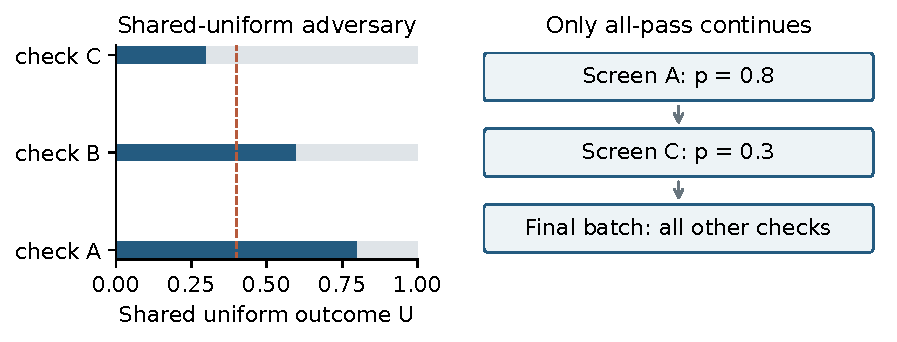
\includegraphics[width=\textwidth]{figures/structure.pdf}
\caption{Left: the shared-uniform coupling nests pass events. At $U=0.4$,
the check with marginal $0.3$ fails while the other illustrated checks pass.
Right: an example of the optimal-policy normal form. Arrows denote all-pass
continuation; a failure terminates. The illustration does not specify costs
and does not assert that these particular screening checks are optimal.}
\label{fig:structure}
\end{figure}

\section{The Probability-Record Normal Form}
\begin{theorem}[Record normal form]\label{thm:normal}
There exists an optimal policy of the form
\begin{equation}
(\{i_1\},\ldots,\{i_\ell\},N\setminus\{i_1,\ldots,i_\ell\}),
\quad
1>p_{i_1}>\cdots>p_{i_\ell},
\label{eq:normal}
\end{equation}
where $0\leq\ell\leq n-1$. The final batch is nonempty.
\end{theorem}
\begin{proof}
Start with an optimal ordered partition. In every nonfinal batch retain one
test whose marginal is smallest in that batch. Move all other tests of that
batch to the final batch. This preserves the minimum marginal after every
nonfinal batch, since a minimum representative remains. It preserves the
number and setup charges of batches. A moved test is charged at the final
batch's survival probability instead of its original, weakly larger survival
probability. Nonnegative additive costs therefore cannot increase the value.
This yields singleton nonfinal batches and a nonempty final batch.

Now consider a singleton whose marginal is at least the current prefix
minimum, taking the initial minimum as one. Move that singleton to the final
batch and remove its batch. The prefix minimum does not change, so all
remaining continuation probabilities stay the same. The removed setup charge
is nonnegative, and the moved test cost is paid at weakly smaller survival.
Repeating this operation eliminates all nonrecords, including marginal-one
screens and equal-marginal screens. The remaining singleton marginals
strictly decrease. Every transformation preserves a valid ordered partition,
so applying it to an optimum proves the claim.
\end{proof}
The proof allows zero costs, zero setup, tied marginals, and probabilities
zero or one. An unrestricted final batch is essential, because capacity
can prevent deferral. Additive costs are also essential; general subadditive
costs need not preserve the comparison.

The normal form is more specific than sorting every test by probability.
Costs determine which records to select, and many tests can be deferred.
For example, let
$p=(0.8,0.3,0.7,0.6,0.9,0.95)$,
$c=(1,10,20,30,40,50)$, and $\beta=0.1$.
Screening tests 1 and 2 and then batching the rest costs
$1.1+0.8(10.1)+0.3(140.1)=51.21$.
Screening test 2 first and batching the rest costs
$10.1+0.3(141.1)=52.43$.
The cheap first screen can be useful even though it is not the smallest
marginal.

\section{An Exact Lower-Envelope Algorithm}
Set $C=\sum_i c_i$, and let a nonempty screening prefix have final marginal
$q=p_{i_\ell}$. Put $p_{i_0}=1$. Expanding~\eqref{eq:risk} gives
\begin{equation}
R_p(\pi)=q(C+\beta)+
\sum_{t=1}^{\ell}
 \left[p_{i_{t-1}}\beta+(p_{i_{t-1}}-q)c_{i_t}\right].
\label{eq:decompose}
\end{equation}
For fixed $q$, the second term is a shortest-path objective on a directed
acyclic graph of strictly decreasing probabilities. A source $0$ has
probability one and distance zero. For every $j$ with $q\leq p_j<1$, define
\begin{equation}
d_q(j)=\min_{\substack{i=0\text{ or }p_i>p_j\\i\text{ already processed}}}
 \{d_q(i)+p_i(\beta+c_j)-qc_j\}.
\label{eq:dag}
\end{equation}
Process vertices in decreasing probability, and use the best terminal vertex
with $p_j=q$. Compare all distinct $q<1$ with the no-screen policy of value
$C+\beta$.

\paragraph{Nonempty terminal batch.}
Equation~\eqref{eq:decompose} presumes that at least one test remains after
the screens. The unrestricted graph can also produce a path containing all
$n$ tests. Truncating its last vertex makes that vertex the final singleton
batch. The physical schedule is unchanged, and its cost is the graph
expression minus the fictitious final setup $q\beta$. The implementation
evaluates the reconstructed ordered partition directly. This cannot introduce
an infeasible policy. Conversely, every valid normal-form optimum is represented
by its final $q$ and path. Thus taking the best reconstructed policy is exact,
even when $\beta=0$ or ties occur. In particular, retaining only a shortest
path for each terminal vertex is sufficient: reconstructing and, if necessary,
truncating that path never increases its graph objective.

\begin{theorem}[Algorithmic complexity]\label{thm:algorithm}
The unrestricted problem can be solved with $O(n^2\log n)$ arithmetic
operations and $O(n)$ auxiliary storage, excluding the input and output.
For rational input an exact rational implementation is possible.
\end{theorem}
\begin{proof}
First, direct predecessor scans in~\eqref{eq:dag} give $O(n^2)$ operations
for each of at most $n$ terminal marginals. They require only distances and
one predecessor per vertex. The normal form and the terminal-batch treatment
above prove exactness.

For the faster implementation, associate predecessor $i$ with the line
$L_i(x)=d_q(i)+p_i x$. A query at $x=\beta+c_j$ returns its minimum; subtract
$qc_j$ to obtain $d_q(j)$. The source contributes $L_0(x)=x$.
Lines arrive in decreasing slope order. All vertices in an equal-probability
group query the envelope \emph{before} the group is inserted, enforcing the
strict predecessor inequality. Only the group's smallest intercept can
matter for later queries.

Maintain the lower envelope as lines with increasing intersection
breakpoints. When inserting a smaller-slope line, pop the last line while
its new intersection is no greater than its existing breakpoint. Each line
is inserted once and popped at most once. Binary search over breakpoints
answers arbitrary-order queries in $O(\log n)$ time. This gives
$O(n\log n)$ operations per $q$. Reconstructing all terminal candidates
costs $O(n^2)$ across all $q$, since there are at most $n$ terminal vertices
in total and each path has length at most $n$. Storage is reused between
terminal marginals.
\end{proof}
The bound counts arithmetic operations and comparisons. It is not a claim
that arbitrary-precision rational operations take constant bit time.
Path weights, distances, and intersections have polynomial bit length in
the rational input encoding, so the exact version remains polynomial.
The implementation supports Python rational numbers for verification and
floating point for timing and replay. Nearly coincident slopes are included
in the exact-arithmetic tests.

The artifact implements the cubic reference, lower envelope, subset oracle,
and ambiguity LP. It supports exact rational verification and double-precision
experimentation. A probability-zero check remains in the partition even when
its continuation branch has zero probability.

\subsection{Zero setup: faster optimization and operational refinement}
\begin{theorem}\label{thm:zero}
When $\beta=0$, an optimal singleton policy can be computed in
$O(n\log n)$ arithmetic operations and $O(n)$ storage. Splitting the residual
batch of any robust-optimal normal-form policy into singletons preserves its
robust optimum and weakly reduces its cost on every Boolean outcome.
\end{theorem}
\begin{proof}
With no setup charge, splitting a batch never increases committed cost on
any outcome: the split policy pays only a prefix of that batch when it fails.
Consequently an optimal singleton policy exists. Let $q=\min_i p_i$.
In a singleton schedule, move each test that fails to establish a strict
probability record before the first global-minimum test to after that test.
Removing it leaves all earlier prefix minima unchanged and charges its cost
at $q$ rather than a weakly larger survival probability. Repeating yields a
strict record path ending at $q$, followed by the remaining tests. Thus only
one terminal marginal, $q$, is needed in~\eqref{eq:dag}. Its lower-envelope
pass costs $O(n\log n)$. Reconstruct only the best terminal path once; append
all remaining tests as singletons. If $q=1$, every singleton order is optimal.

For the second claim, the splitting argument gives pointwise domination.
Its robust value cannot exceed the original optimum, and cannot be below
the optimum, so equality holds. Within the fixed residual tail, ordering by
$c_i/(1-p_i)$ minimizes independent-law cost by adjacent exchanges; tests
with $p_i=1$ may be placed last. This orders only the fixed tail, not all
robust-optimal prefixes.
\end{proof}
The faster algorithm and the refinement of the general optimizer can choose
different robust-optimal prefixes. Neither is claimed to minimize nominal
cost over the entire set of robust optima. Our reported policies use the
cubic reference's frozen prefix and apply the refinement at zero setup;
positive-setup policies are unchanged. This separates an implementation
choice from a mathematical guarantee.

The normal form is an \emph{existence} theorem for the pure robust objective,
not a complete description of its optima or a nominal--robust frontier.
For example, take three tests with $p_i=1/2,c_i=1,\beta=0$.
Every singleton order has robust cost $2$ and independent cost $7/4$.
A record-prefix policy can use at most one screen: its best robust and
independent costs are both $2$. Hence for every $0\leq\lambda<1$, the mixed
objective $\lambda R+(1-\lambda)E_{\rm ind}$ strictly prefers the singleton
policy to every record-form policy. An arbitrarily small nominal weight
therefore invalidates restricting optimization to the normal form.
The refinement avoids this particular degeneracy without asserting a
polynomial algorithm for that different objective.

\section{Dependence Risk and Marginal Uncertainty}
\begin{theorem}[Unbounded independence-design loss]\label{thm:gap}
The robust approximation ratio of an independence-optimal policy is
unbounded, even when $\beta=0$.
\end{theorem}
\begin{proof}
Take $m\geq2$ tests with $c_i=1,p_i=1/2$ and one test $z$ with
$c_z=3,p_z=\varepsilon=m^{-2}$. With zero setup, splitting a batch into
singletons cannot increase expected cost. Under independence, exchanging
adjacent singleton tests orders them by increasing $c_i/(1-p_i)$.
The cheap tests have ratio 2 and $z$ has ratio $3/(1-\varepsilon)>3$;
thus an independent optimum places all cheap tests first. Its robust value
is $1+(m-1)/2+3/2=m/2+2$.

Under the record normal form, at most one cheap test can screen, since their
marginals are equal. For $m\geq2$, screening a cheap test, then $z$, then
batching the remaining cheap tests has value
$1+3/2+\varepsilon(m-1)$.
Screening only a cheap test has value $m/2+2$; screening only $z$ has value
$3+\varepsilon m$; using no screens costs $m+3$. These exhaust the
record patterns and establish the stated policy as optimal, allowing a
tie when $m=2$. Its value stays bounded while $m/2+2$ diverges.
\end{proof}
This is a model-separation result. It does not predict that an actual
industrial workload will realize the extremal dependence.

\begin{proposition}[Intervals and sensitivity]\label{prop:uncertainty}
If only $p_i\in[l_i,u_i]$ is known and dependence is unrestricted, the robust
optimization problem is exactly the fixed-marginal problem at $u$.
For fixed costs and $L=C+n\beta$,
\begin{equation}
|R_p(\pi)-R_{p'}(\pi)|\leq L\|p-p'\|_\infty,
\qquad
|\OPT(p)-\OPT(p')|\leq L\|p-p'\|_\infty.
\label{eq:lipschitz}
\end{equation}
If $\widehat{\pi}$ is optimal at $\widehat p$ and
$\|p-\widehat p\|_\infty\leq\delta$, then
$R_p(\widehat{\pi})-\OPT(p)\leq2L\delta$.
\end{proposition}
\begin{proof}
Every nonempty-prefix minimum is coordinatewise nondecreasing. Its maximum
over the box occurs at $u$, and the shared-uniform law at $u$ is feasible,
proving the interval statement. The minimum of a fixed subset is
1-Lipschitz in the sup norm. The total unweighted batch charges are at most
$C+n\beta$, proving the first inequality in~\eqref{eq:lipschitz}.
Taking minima over policies gives the second. Inserting
$R_{\widehat p}(\widehat{\pi})=\OPT(\widehat p)$ between the two objectives
gives the regret bound.
\end{proof}

For $T$ fully observed independent and identically distributed episodes,
let $\widehat p_i$ be the sample pass rate. A one-sided Hoeffding bound
\cite{hoeffding1963} and a union bound give simultaneous upper bounds
\[
u_i=\min\left\{1,\widehat p_i+
\sqrt{\frac{\log(n/\alpha)}{2T}}\right\}
\]
with probability at least $1-\alpha$. On that event, a policy optimized at
$u$ has expected cost under the true joint law at most $R_u(\pi)$.
Independence is required across episodes, not among tests within an episode.
This certificate does not apply directly to drift, adaptive sampling, or
censored logs. We therefore do not attach it to the chronological replay.
The Lipschitz bound is global and may be loose, especially when many tests
have high estimated pass probabilities.

\section{Capacity: A Complexity Boundary and CP Formulation}
Suppose tests have positive integer loads $a_i$, and each batch must satisfy
$\sum_{i\in B}a_i\leq A$. The universal least-favorable law remains valid,
but the normal form can fail. With four tests, $p_i=1/2,c_i=1,\beta=10$,
unit loads, and capacity two, two size-two batches cost
$12+\tfrac12(12)=18$. A singleton-prefix policy with a final batch of size
at most two requires at least two singleton screens and costs at least
$11+\tfrac12(11)+\tfrac12(12)=22.5$.

\begin{theorem}\label{thm:hard}
Capacity-constrained marginally robust batch testing is strongly NP-hard.
\end{theorem}
\begin{proof}
Reduce from 3-Partition with $3m$ item sizes $a_i$, total $mA$, and
$A/4<a_i<A/2$. Set every $p_i=1/2$, every $c_i=0$, and $\beta=1$.
A feasible partition into $k$ batches has robust cost
$1+\tfrac12(k-1)$. It has cost at most $(m+1)/2$ if and only if
the items fit in at most $m$ batches of capacity $A$. Total load forces
exactly $m$ full batches, and the size restrictions force exactly three
items per batch. This is equivalent to the 3-Partition instance.
The reduction uses fixed probabilities and fixed costs, preserving strong
NP-hardness.
\end{proof}
The hardness is inherited from packing; it does not establish hardness for
unit loads or every capacity variant.

For integer-grid probabilities $p_i=u_i/P$ and integer costs, we use a
direct CP-SAT model. There are $n$ potential stages. Binary $x_{ib}$
assigns each test to exactly one stage; binary $y_b$ indicates a nonempty
stage. Let $s_b$ be the scaled survival before stage $b$, and $h_b$ its charge:
\begin{align}
&\sum_b x_{ib}=1,\quad
y_b\leq\sum_i x_{ib}\leq n y_b,\quad y_b\geq y_{b+1},
\quad \sum_i a_i x_{ib}\leq A,\label{eq:cp1}\\
&s_0=P,\quad
s_{b+1}=\min\left(s_b,\min_i\{P-(P-u_i)x_{ib}\}\right),\label{eq:cp2}\\
&h_b=\beta y_b+\sum_i c_i x_{ib},\qquad
z_b=s_b h_b,\qquad
\min\ \frac1P\sum_b z_b.\label{eq:cp3}
\end{align}
Empty stages trail nonempty stages and contribute zero. Equations
\eqref{eq:cp2}--\eqref{eq:cp3} use native minimum and integer product
constraints. The model has $O(n^2)$ assignment variables. Its objective
exactly equals~\eqref{eq:risk} on the input probability grid. Scaling or
rounding probabilities before optimization changes the input problem and
must be reported. We use generated exact-grid inputs and verify the objective
by independent policy evaluation.

The formulation uses standard CP-SAT capabilities \cite{perron2023}; it is
not a new general constraint-solving technique. Removing capacity gives
the unrestricted RecordBatch value as a valid lower bound. The present
implementation records that bound for comparison, without claiming a
specialized branch-and-bound method or a speed advantage over existing
batch-testing solvers.

\section{Computational Evaluation}
All code, seeds, generated instances, derived replay panels, results, and
figure scripts accompany the manuscript. Solver versions and machine
information are recorded separately. Reported wall times describe one
machine and implementation; they are not complexity proofs. Unless explicitly
using rational arithmetic, computations use double precision.

\subsection{Independent implementation checks}
The test suite checks multiple levels of the claim:
\begin{itemize}
\item 648 small rational grid instances and 270 seeded random rational
instances compare both unrestricted algorithms with a subset dynamic program.
\item 70 instances compare prefix-min evaluation with a full $2^n$-outcome
linear program over all joint probabilities, including marginal constraints.
\item 18 capacity instances compare CP-SAT optima with the capacity-aware
subset oracle.
\item 15 near-coincident-probability instances compare the envelope and
cubic algorithms using exact rational arithmetic.
\item Seven instances check empirical-joint subset optimization; seven check
the unbounded-gap family. Another 160 rational cases check the specialized
zero-setup algorithm and pointwise refinement on every Boolean outcome.
\item 120 near-one floating-point instances re-evaluate returned policies
with exact rational arithmetic, across small setup and cost scales. A
three-test example checks failure of the normal form for mixed objectives.
\end{itemize}
The subset oracle enumerates every possible next nonempty residual subset,
using the unnormalized survival probability of the already tested set.
It does not use the record normal form. The ambiguity LP independently
computes each Boolean outcome's policy cost before optimizing its probability.
These are implementation checks, not substitutes for the proofs or an
independent scientific replication.

\subsection{Synthetic dependence-risk experiments}
The 480-instance design crosses $n\in\{8,12\}$, twenty replicates, three marginal
families, and four setup ratios
$\beta/\overline c\in\{0,0.1,1,5\}$. Marginal families are uniform on
$[0.05,0.5]$, $[0.05,0.95]$, and $[0.8,0.999]$, respectively.
A single fixed random seed drives the full grid.
Costs are positive integer draws. We compare RecordBatch with an
\emph{exact} independent-law subset-DP optimizer (IndependentDP), not merely
a greedy independence heuristic. Additional baselines are one full batch
and singleton ratio ordering. For each schedule we compute both its exact
worst-case cost and its exact expected cost under independence.

\begin{table}[t]
\caption{Synthetic results, 120 instances per setup ratio. Entries are medians
of instance-level percentages. Positive worst-case saving favors RecordBatch;
positive nominal premium is its cost under the independent law.}
\label{tab:synthetic}
\centering
\begin{tabular}{rrrr}
\toprule
$\beta/\overline c$ & Worst-case saving (\%) & Nominal premium (\%) &
Prefix screens\\
\midrule
0 & 0.003 & 0.01 & 2\\
0.1 & 5.35 & 50.56 & 2\\
1 & 16.11 & 27.34 & 1\\
5 & 16.23 & 13.42 & 1\\
\bottomrule
\end{tabular}
\end{table}
Table~\ref{tab:synthetic} reports savings
$100(R_p(\pi_{\rm ind})-R_p(\pi_{\rm rec}))/R_p(\pi_{\rm ind})$
and independent-law premium
$100(E_{\rm ind}C(\pi_{\rm rec})/E_{\rm ind}C(\pi_{\rm ind})-1)$.
The largest observed worst-case saving is 35.10\%.
At positive setup, nominal premiums remain substantial. At zero setup,
refining the residual batch reduces the median nominal premium from 49.64\%
to 0.01\%, preserving every robust value. Thus a poor representative of a
robust tie can create an avoidable premium; it must not be interpreted as
an inherent insurance price. The near-zero median worst-case saving at zero
setup also rules out a blanket claim that dependence protection is valuable.
Theorem~\ref{thm:gap} is an adversarial family, not a typical-case statement.

\begin{figure}[t]
\centering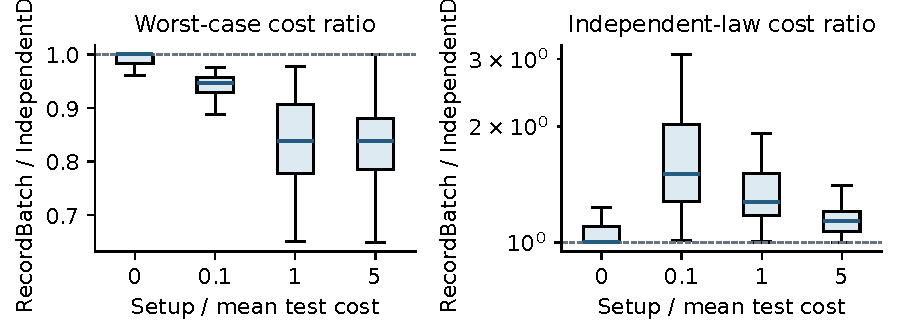
\includegraphics[width=\textwidth]{figures/synthetic.pdf}
\caption{Synthetic cost ratios against exact IndependentDP, grouped by setup
ratio. Boxes show interquartile ranges and medians; whiskers follow the
standard 1.5-IQR rule, with outlier markers suppressed. Left: worst-case
cost, where ratios below one favor RecordBatch. Right: independent-law
cost on a logarithmic scale, exposing its nominal premium.}
\label{fig:synthetic}
\end{figure}

\subsection{Scaling and the capacity extension}
The paired timing benchmark draws five instances per size with a fixed seed,
$p_i$ uniform on $[0.05,0.95]$, $c_i$ uniform integer on $[1,100]$, and
$\beta=10$. Both unrestricted implementations run on the same inputs up
to $n=512$; the envelope implementation also runs at $n=1024,2048$.
At $n=512$, median times are 5.587 seconds for the cubic reference and
0.237 seconds for the envelope, approximately a 23.6-fold reduction.
At $n=2048$, the envelope median is 3.804 seconds.
Figure~\ref{fig:scaling} reports the measured range as well as the median.
An additional 480 synthetic comparisons agree between implementations to
absolute error below $10^{-8}$. The zero-setup algorithm is measured separately
on five instances per size, with seed 120727 and the same marginal and cost
families. Median times are 0.0057 seconds at $n=2048$ and 0.093 seconds at
$n=32768$. These use the specialized objective with $\beta=0$, so they are
not a direct speed comparison with the positive-setup benchmark.

\begin{figure}[t]
\centering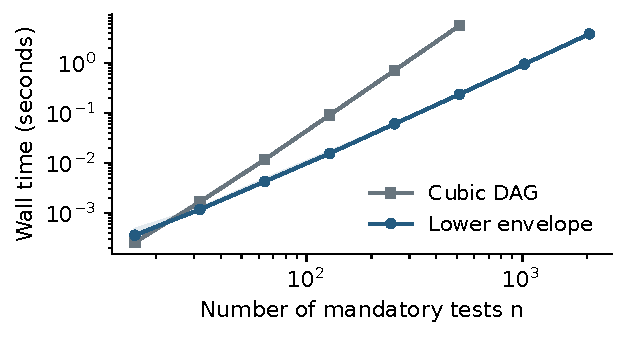
\includegraphics[width=.77\textwidth]{figures/scaling.pdf}
\caption{Paired wall-time measurements, five seeded instances per size.
Lines show medians and shading shows minimum to maximum. The cubic reference
is stopped after $n=512$. The theorem establishes an arithmetic-operation
bound; these measurements describe the supplied Python implementation.}
\label{fig:scaling}
\end{figure}

Capacity experiments use exact probability grids and one CP-SAT worker.
The initial 30 cases at $n=8,12,16$ all solve to proven optimality.
Ten additional cases at $n=24,32$ use a ten-second limit per case.
All five $n=24$ cases and two of five $n=32$ cases solve to optimality.
The other three return feasible solutions with relative solver gaps
25.63\%, 14.08\%, and 20.36\%, using
$(\mathrm{incumbent}-\mathrm{bound})/\mathrm{incumbent}$.
Thus 37 of 40 cases are proved optimal. These small synthetic cases establish
that the extension is executable; they do not establish scalability on
industrial capacity-constrained problems.

\subsection{Chronological replay on industrial test logs}
We use the public Westermo dataset \cite{strandberg2022}, pinned to repository
commit \texttt{31ca0ab8} (the full hash is recorded in the artifact).
The source contains 1,063,915 verdict rows. We retain nightly sessions
(type N), main releases (M), and verdicts 0 or 1, leaving 472,447 rows.
For each of nine systems, the first 60\% of sessions form the chronological
training period. The twelve most frequently observed training tests define
that system's panel, with ascending test identifiers breaking frequency ties.
Only sessions observing all twelve selected tests are retained for marginal
estimation or replay. Multiple results for one session--test pair are combined
by maximum verdict, treating any observed failure as failure.
The resulting panels contain 1,693 complete training sessions and 797 complete
held-out sessions. Systems must have at least 30 complete training and 20
complete test sessions. Counts and selected identifiers are supplied per system.

Pass probabilities are estimated from complete training panels. Fixed test
costs are median training durations for the selected tests, floored at one
duration unit. We vary a \emph{modeled} setup charge over
$\beta/\mathrm{median}(c)\in\{0,0.1,1,5\}$; the logs do not identify a
causal setup cost for our hypothetical batching intervention.
All policies are frozen before the held-out period. Baselines include
IndependentDP, singleton ratio ordering, a full batch, and an empirical-joint
subset-DP policy learned from the same complete training episodes.
The last baseline can exploit observed training dependence, though estimating
its subset survival probabilities is data intensive.

\begin{figure}[t]
\centering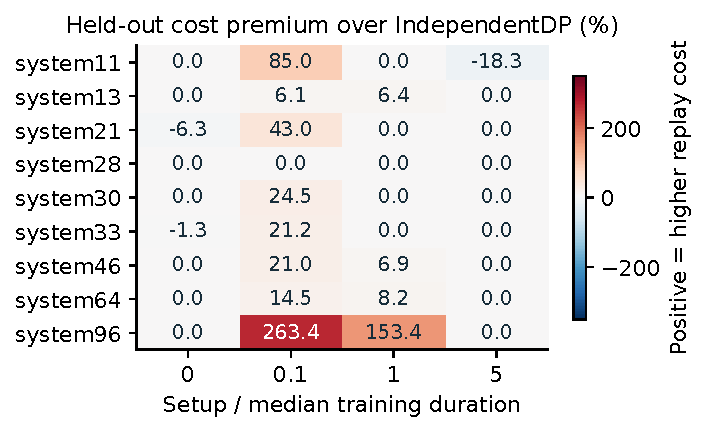
\includegraphics[width=.88\textwidth]{figures/replay.pdf}
\caption{Chronological held-out replay: percentage cost premium of RecordBatch
over IndependentDP in each of 36 system--setup configurations. Positive
values mean higher replay cost. Each cell reuses the corresponding system's
held-out sessions; cells are not independent experimental replicates.}
\label{fig:replay}
\end{figure}

Figure~\ref{fig:replay} shows the central operational limitation.
After zero-setup refinement, RecordBatch has lower mean replay cost in three
configurations, ties in twenty, and costs more in thirteen. Its median
configuration-level premium over IndependentDP is zero; the largest is
263.41\% at positive setup. The unrefined zero-setup policy cost 689.44 on
system96 and 380.00 on system11; refinement reduces these to 153.78 and
116.00, respectively, equal to IndependentDP. The zero-setup ablation retains
both policies and per-configuration results. These changes illustrate why
robust optimality alone cannot justify an arbitrary robust tie for deployment.
Positive-setup conservatism persists. Large modeled setup charges often make
the policies choose the same full batch. The 36 related cells are not treated
as independent observations for significance testing.

Table~\ref{tab:replay} includes all additional baselines. An empirical joint
model sometimes improves over independence, but sometimes transfers poorly
to the held-out period. Its zero median premium is not evidence of a calibrated
future-risk guarantee. Ratios are normalized within configuration before
aggregation, avoiding a pooled average across systems with different cost scales.

\begin{table}[t]
\caption{All replay baselines relative to IndependentDP. Premiums are medians
over 36 configurations; lower/equal/higher counts use mean held-out cost within
each configuration. These are descriptive, related comparisons.}
\label{tab:replay}
\centering
\begin{tabular}{lrrrr}
\toprule
Policy & Premium (\%) & Lower & Equal & Higher\\
\midrule
RecordBatch & 0.00 & 3 & 20 & 13\\
EmpiricalDP & 0.00 & 6 & 19 & 11\\
AllBatch & 7.55 & 3 & 12 & 21\\
RatioSerial & 0.84 & 11 & 7 & 18\\
\bottomrule
\end{tabular}
\end{table}

Replay charges a batch's fixed modeled cost if all previous batches pass in
that logged episode. It preserves the observed outcome vector and changes
only the evaluation schedule. This requires outcome invariance under schedule
changes, an assumption rather than a result established by the logs.
Complete-case selection can bias the included population; the source execution
order can also affect which tests were observed. Chronological drift is
visible, including selected tests with training pass rate one that fail later.
Point-estimated marginal robustness protects neither against this drift nor
against marginal estimation error. A certificate would require defensible
intervals or a suitable temporal model, rather than applying the iid guarantee
to these sessions. The replay therefore supplies evidence of conservatism
and model mismatch, not evidence of production savings or of a valid
out-of-sample risk bound.

\section{Practical Implications, Limitations, and Conclusion}
The exact optimizer is useful when dependence protection is an explicit
operational requirement. Examples include mandatory software or data
validation gates whose individual pass rates are available but whose shared
failure structure is not trusted. Its output is simple to execute: singleton screens followed by one residual
batch, with the tail split when setup is zero. A deployment can
compare its robust cost with a nominal schedule and expose that insurance
price before choosing a policy. Commercial use still requires measuring
setup and test costs, checking schedule invariance, and deciding whether
unrestricted dependence is an appropriate uncertainty model.

The principal mathematical limitation is also the source of tractability:
under unrestricted dependence, successful nonrecord checks convey no further
worst-case reduction in continuation probability. Pairwise information, a
restricted family of failure mechanisms, or a learned joint model can make
such checks informative again. The record proof then need not hold.
Resource capacity already breaks it, as the counterexample and hardness
reduction show. Parallel elapsed time, imperfect checks, dynamic outcomes,
batch-dependent costs, and adaptive information acquisition are outside the
current theorem.

This work separates three issues that are easy to conflate: a classical
least-favorable coupling, a policy-optimization structure for a particular
cost model, and the empirical desirability of that cost-risk objective.
For the second issue, RecordBatch gives an exact polynomial solution and a
clear capacity boundary. For the third, the evidence is mixed by design:
synthetic risk reductions coexist with industrial replay premiums.
Further work should investigate intermediate dependence information and
temporal marginal uncertainty while retaining explicit guarantees and
auditable schedules.

\paragraph{Reproducibility and author contributions.}
Source, exact-oracle checks, input instances, derived data, results, and figure
scripts are available at \url{https://github.com/shi1720/recordbatch-artifact}.
Shivam Gupta set the research objectives, critically reviewed the proofs,
code, data, and conclusions, and directed revision toward novelty and practical
relevance. No independent external replication is claimed.

\paragraph{Acknowledgements and generative assistance.}
OpenAI Codex was used on 11--12 October 2026 for research exploration,
algorithm and proof drafting, implementation, experimental execution,
figure preparation, and manuscript drafting and revision, including substantive
research reasoning. Prompts requested an original CPAIOR study with code,
experiments and literature review, then critical review and improvement of
RecordBatch's novelty and practicality. Exact model/build metadata was not
recorded. The author critically reviewed the research and is responsible for
the final claims, interpretation, and submission.

\begin{thebibliography}{14}
\bibitem{agrawal2012}
Agrawal, S., Ding, Y., Saberi, A., Ye, Y.:
Price of correlations in stochastic optimization.
Operations Research \textbf{60}(1), 150--162 (2012).
\doi{10.1287/opre.1110.1011}
\bibitem{daldal2017}
Daldal, R., \"Ozl\"uk, \"O., Sel\c{c}uk, B., Shahmoradi, Z., \"Unl\"uyurt, T.:
Sequential testing in batches.
Annals of Operations Research \textbf{253}, 97--116 (2017).
\doi{10.1007/s10479-016-2345-7}
\bibitem{ghuge2026}
Ghuge, R., Moondra, J., Singh, M.:
Stochastic function certification with correlations.
arXiv preprint arXiv:2604.02611 (2026).
\doi{10.48550/arXiv.2604.02611}
\bibitem{harris2025}
Harris, B., Nagarajan, V., Tan, R.:
Sequential testing with subadditive costs.
In: Integer Programming and Combinatorial Optimization.
LNCS, vol.~15620, pp.~283--296. Springer (2025).
\doi{10.1007/978-3-031-93112-3_21}
\bibitem{hoeffding1963}
Hoeffding, W.:
Probability inequalities for sums of bounded random variables.
Journal of the American Statistical Association \textbf{58}(301), 13--30 (1963).
\doi{10.1080/01621459.1963.10500830}
\bibitem{kaplan2005}
Kaplan, H., Kushilevitz, E., Mansour, Y.:
Learning with attribute costs.
In: Proceedings of the 37th Annual ACM Symposium on Theory of Computing,
pp.~356--365. ACM (2005).
\doi{10.1145/1060590.1060644}
\bibitem{perron2023}
Perron, L., Didier, F., Gay, S.:
The CP-SAT-LP solver (invited talk).
In: 29th International Conference on Principles and Practice of Constraint
Programming. LIPIcs, vol.~280, pp.~3:1--3:2 (2023).
\doi{10.4230/LIPIcs.CP.2023.3}
\bibitem{segev2022}
Segev, D., Shaposhnik, Y.:
A polynomial-time approximation scheme for sequential batch testing of
series systems.
Operations Research \textbf{70}(2), 1153--1165 (2022).
\doi{10.1287/opre.2019.1967}
\bibitem{strandberg2022}
Strandberg, P.E.:
The Westermo test results data set.
arXiv preprint arXiv:2211.13622 (2022).
Dataset: \url{https://github.com/westermo/test-results-dataset}
\bibitem{tan2025}
Tan, R., Xu, A., Nagarajan, V.:
A general framework for sequential batch-testing.
Operations Research Letters \textbf{63}, 107348 (2025).
\doi{10.1016/j.orl.2025.107348}
\bibitem{tan2026}
Tan, R., Nagarajan, V.:
Distributionally robust $k$-of-$n$ sequential testing.
arXiv preprint arXiv:2603.23705 (2026).
\doi{10.48550/arXiv.2603.23705}
\bibitem{unluyurt2004}
\"Unl\"uyurt, T.:
Sequential testing of complex systems: a review.
Discrete Applied Mathematics \textbf{142}, 189--205 (2004).
\doi{10.1016/j.dam.2002.08.001}
\bibitem{unluyurt2025}
\"Unl\"uyurt, T.:
Sequential testing problem: a follow-up review.
Discrete Applied Mathematics \textbf{377}, 356--369 (2025).
\doi{10.1016/j.dam.2025.07.039}
\bibitem{yang2024}
Yang, F., Hermans, B., Zufferey, N., Leus, R.:
Sequential testing in batches with resource constraints.
Expert Systems with Applications \textbf{256}, 124858 (2024).
\doi{10.1016/j.eswa.2024.124858}
\end{thebibliography}
\end{document}
